%!TEX root = ./pres.tex

\begin{frame}{Технический момент: используемые обозначения}
    \begin{table}
        \begin{center}
            \begin{tabular}{|c|c|}
                \hline
                $Q$ &квазигруппа с операцией $\circ$ \\
                \hline 
                $k$ & размер множества $Q$, $k = \lvert Q \rvert$, значность логики \\
                \hline
                $\EE_k$ & множество $\{0, \ldots, k-1 \}$ (обычно предполагаем $\EE_k = \ZZ_k$) \\
                \hline
                $\ff$ & семейство (набор) функций $\ff = (f_1, \ldots, f_n)$, \\
                      & $\ff \colon Q^n \to Q^n$ \\
                \hline 
                $f_i$ & $i$-я функция семейства $\ff$ \\
                \hline
                $n$ & размер семейства \\
                \hline
                $Func(Q)$ & множество функций $f \colon Q \to Q$ \\
                \hline 
                $Perm(Q)$ & множество подстановок (биекций) на $Q$ \\
                \hline
            \end{tabular}
        \end{center}
    \end{table}
\end{frame}


\begin{frame}{Еще технический момент}

    \begin{myexample}{Примеры/определения}
        Как правило, НЕ мои.
    \end{myexample}

    \begin{mypropos}{Утверждения}
        Тоже не мои.
    \end{mypropos}

    \begin{mytheorem}{Леммы-теоремы-утверждения}
        Мои.
    \end{mytheorem}

    Где не мои~--- приводятся ссылки на работы.
    Если в тексте есть упоминание Теоремы $\mathsf{X}$, то номер $\mathsf{X}$ взят из диссертации.

\end{frame}


\section{Введение: зачем исследуем?}


\begin{frame}{ \textquote{Обычная} криптография}
    В криптографии широко используются различные алгебраические структуры:
    \begin{coloritemize}
        \item поля: $\FF_q$;
        \item коммутативные группы: $\FF_q^*$, $\EE(\FF_q)$;
        \item кольца (коммутативные, ассоциативные, с единицей): $\ZZ$, $\ZZ_n$;
        \item коды (векторные подпространства над конечными полями), решетки~\footcite{pqcrypto}, ...
    \end{coloritemize}
\end{frame}


\begin{frame}{ \textquote{Необычная} криптография}
    При этом в исследовательской литературе предлагаются к рассмотрению и более \textquote{экзотические} структуры, например:
    \begin{coloritemize}
        \item модули более общего вида~\footcite{nechaev95};
        \item \textbf{некоммутативные} группы и алгебры (например, группы кос, алгебры матриц, алгебра кватернионов и так далее)~\footcite{myasnikov2011non, romankov, moldovyan};
        \item \textbf{неассоциативные структуры}: квазигруппы, квазигрупповые кольца и т.д~\footcite{glukhov, artamonov18, markov2020nonassociative}.
    \end{coloritemize}
    Именно на последние мы и посмотрим чуть подробнее.
\end{frame}


\begin{frame}{Квазигруппа}
    \begin{myexample}{Квазигруппа, \defn~1}
        Множество $Q$ с заданной на нём бинарной операцией
        \(
          \circ \colon Q \times Q \to Q, 
        \)
        со следующим свойством: для любых $a, b \in Q$ существуют единственные $x, y \in Q$, такие что:
        \[
          a \circ x = b, \qquad y \circ a = b.
        \]
        \footcitetext{belousov, keedwell}
    \end{myexample}

    \pause
    Другими словами, операции \textbf{левого} $L_a$ и \textbf{правого} $R_a$ умножения (сдвиги)
    \begin{gather*}
        L_a \colon Q \to Q,\, L_a(x) = a \circ x, \; R_a \colon Q \to Q,\, R_a(y) = y \circ a,
    \end{gather*}
    являются биекциями на $Q$.
    
    \pause 
    По сути = группа без ассоциативности и единицы, но \textbf{с сокращением} как слева, так и справа.
\end{frame}


\begin{frame}{Несколько примеров}
    \begin{coloritemize}
        \item $Q$~--- любая группа, например $Q = \ZZ_k$, $\circ = +$; 
        \pause 
        \item $Q = \ZZ_k$, $\circ = -$ (не группа, т.к. $a - (b - c) \ne (a - b) - c$);
        \pause
        \item $(G, \cdot)$~--- группа, $\pi$, $\sigma$, $\tau$~--- подстановки на $G$, тогда можно рассмотреть \textbf{изотоп~\footcite{belousov, keedwell}} (\defn~5):
        \[
            x \circ y = \tau(\pi(x) \cdot \sigma(y)).
        \]
    \end{coloritemize}
\end{frame}


\begin{frame}{Латинский квадрат}
    \begin{coloritemize}
        \item Квадратная таблица размера $k \times k$, заполнена элементами множества $\{ 0, \ldots, k-1 \}$, каждое элемент появляется \textbf{только один раз} в каждом столбце и каждой строке таблицы (\defn~2).
        \item Таблица умножения квазигруппы $Q = \{q_1, \ldots, q_k \}$ (на пересечении $i$-й строки и $j$-го столбца пишем $(q_i \circ q_j) \in Q$) является латинским квадратом.
    \end{coloritemize}

    \begin{columns}[T] % gather columns
        \begin{column}{.2\textwidth}
            \(
                \begin{bmatrix}
                    0 & 1 & 2 & 3 & 4 \\
                    1 & 0 & 3 & 4 & 2 \\
                    2 & 3 & 4 & 0 & 1 \\
                    3 & 4 & 1 & 2 & 0 \\
                    4 & 2 & 0 & 1 & 3 \\
                \end{bmatrix}
            \)
        \end{column}%
        \hfill%
        \begin{column}{.4\textwidth}
            \begin{figure}[h]
                \centering 
                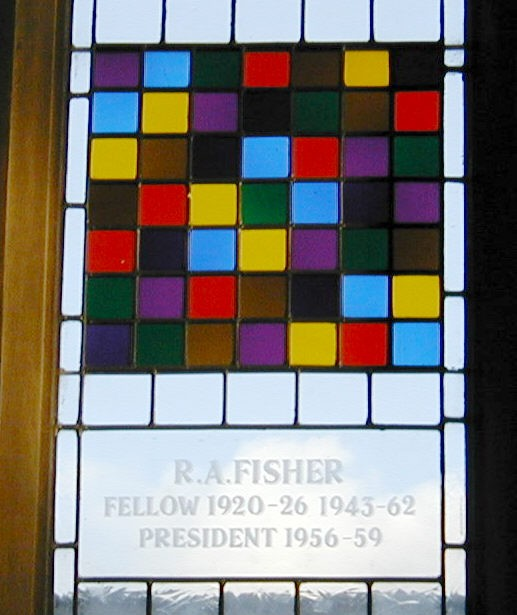
\includegraphics[scale = 0.18]{fisher.jpg}
            \end{figure}
        \end{column}%
    \end{columns}  
\end{frame}


\begin{frame}{Пример: $E$-преобразование}
    Пусть $x_1, \ldots, x_k, \ell \in Q$.
    Определим~\footcite{markovski2017quasigroup} преобразование $E_{\ell}$:
    \[
        E_{\ell}(x_1 \ldots x_k) = y_1 \ldots y_k,
    \]
    \[
        y_1 = \ell \circ x_1, \; y_{i+1} = y_i \circ x_{i+1}.
    \]
    \begin{figure}[h]
        \centering 
        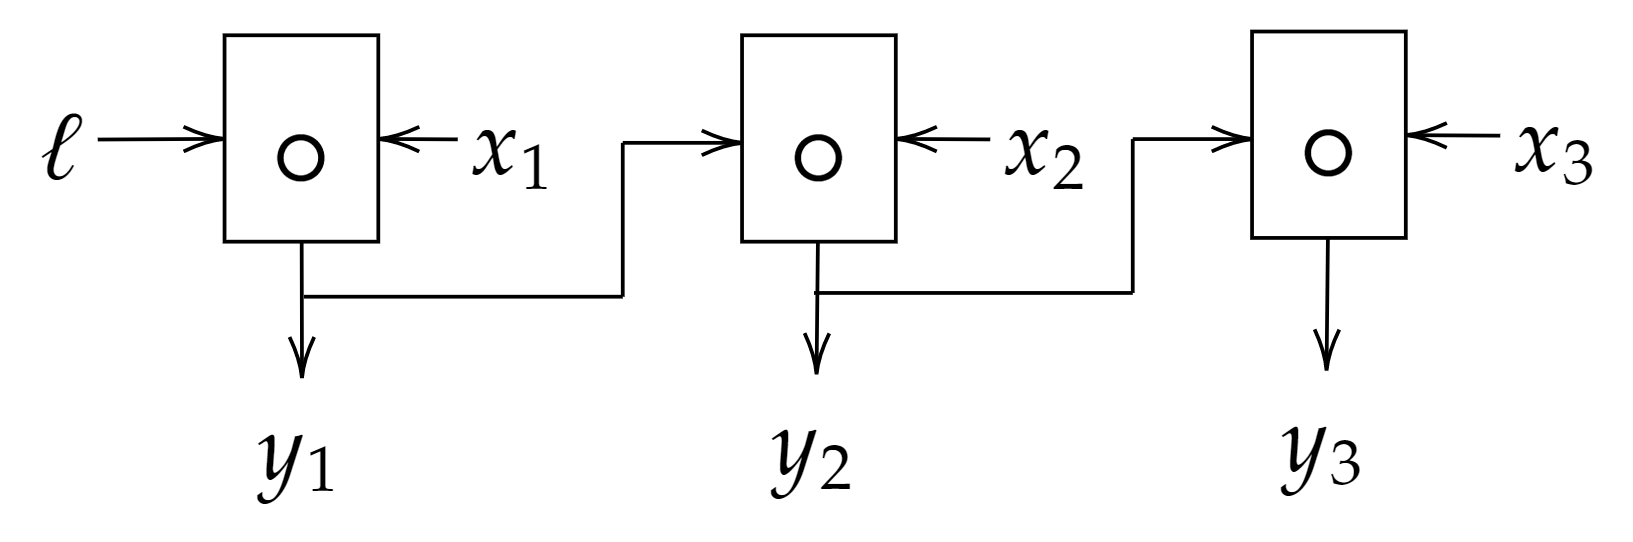
\includegraphics[width = 0.7\linewidth]{etransform.png}
    \end{figure}
\end{frame}


\begin{frame}{Пример: итерации $E$-преобразований}
    \begin{coloritemize}
        \item Можем ввести кратное $E$-преобразование:
        \[
            E_{\ell_1, \ldots, \ell_n}(x) = E_{\ell_1} \left( \ldots \left( E_{\ell_n} (x) \right) \ldots \right), 
        \]
        \item Отображение $E_{a}$ обладает набором <<хороших>> криптографических свойств~\footcite{markovski1999quasigroup, bakeva2011some, markovski2017quasigroup, yash13, yash22, yash22-2}.
    \end{coloritemize}
\end{frame}


\begin{frame}{Механизмы}
    \begin{coloritemize}
        \item ГПСЧ на основе итерации $E$-преобразований~\footcite{dimitrova2004quasigroup, markovski2005unbiased}.
        \item Блочный шифр \textbf{INRU}~\footcite{inru}, $E$-преобразование используется в качестве нелинейного элемента.
        \item  \textquote{Односторонняя функция}~\footcite{gligoroski2008edon, gligoroski2009family, EdonR, EdonRprime} и основанные на ней хэш-функции:
        \[
            R(a_1 \ldots a_n) = E_{a_1} \left( \ldots E_{a_n}(a_1 \ldots a_n) \ldots \right).
        \]
    \end{coloritemize}
\end{frame}


\begin{frame}{Другие предложения (кратко)}
    Основная идея: использовать в качестве нелинейного компонента примитива некоторое квазигрупповое преобразование.
    \begin{coloritemize}
        \item Низкоресурсная (легковесная/lightweight) хэш-функция \textbf{GAGE} и AEAD-алгоритм \textbf{InGAGE} (см.~\url{http://gageingage.org/}, также~\footcite{otte2019gage, gligoroski2019s}).
        \item Поточный шифр \textbf{Edon80}~\footcite{edon80}.
        \item Хэш-функция \textbf{NaSHA}~\footcite{mileva2009quasigroup}.
    \end{coloritemize}
\end{frame}


\begin{frame}{Другие предложения (кратко)-2}
    \begin{coloritemize}
        \item Асимметричные криптопримитивы~--- аналоги пост-квантовых схем (\textbf{multivariate cryptography}~\footcite{preneel}).
        \pause
        \item Основная идея: подобрать такое нелинейное преобразование $\mathcal{P}$, что вычисление $\mathcal{P}$ и $\mathcal{P}^{-1}$ сделать  \textquote{легко}, а затем  \textquote{скрыть} структуру $\mathcal{P}$, взяв обратимые линейные преобразования $\mathcal{S}$ и $\mathcal{T}$ и рассмотрев композицию 
        \(
            \mathcal{F}(x) = \mathcal{S} \left( \mathcal{P} \left(\mathcal{T}(x) \right) \right).
        \)
        \pause 
        \item В работах~\footcite{gligoroski2008public, gligoroski2008multivariate, chen2010multivariate, gligoroski2011mqq} предлагалось рассматривать в качестве нелинейной компоненты $\mathcal{P}$ композицию $E$-преобразований.
        \pause 
        \item В работах~\footcite{mohamed2009algebraic, faugere2015polynomial} предлагаемая система и её модификации были успешно атакованы (решение задачи \textbf{MinRank} с помощью базисов Грёбнера).
    \end{coloritemize}
\end{frame}


\begin{frame}{Другие предложения (кратко)-3}
    \begin{coloritemize}
        \item Схемы~--- аналоги протокола Диффи-Хеллмана выработки общего ключа~\footcite{katyshev14, katyshev18}, гомоморфное шифрование~\footcite{gribov2010construction, gribov15, markov20}: используются \textbf{ППС/ПЛС-группоиды}, \textbf{луповые кольца} над медиальными квазигруппами (изотопы абелевых групп с коммутирующими автоморфизмами).
        \pause
        \item Приложения в теории кодирования~\footcite{nechaev98, nechaev04, couselo2004loop, markov12, markov2020nonassociative}...
        \pause 
        \item и многое другое~\footcite{glukhov, artamonov18, shcherbacov2017elements, chauhan2021quasigroups}.
    \end{coloritemize}
\end{frame}


\begin{frame}{Как задать квазигруппу?}
    \begin{coloritemize}
        \item В общем случае квазигруппа над множеством $Q$ задается таблицей умножения размера $\lvert Q \rvert \times \lvert Q \rvert$; это много.
        \pause 
        \item Случайная генерация (поиск + отсев) квазигрупп из некоторого узкого класса~\footcite{gligoroski2008public, chen2010multivariate}.
        \pause 
        \item Итеративное построение из более \textquote{маленьких} (конструкции наподобие прямых произведений)~\footcite{gribovphd, EdonRprime}.
        \pause 
        \item Изотопы некоторых \textquote{хорошо изученных} групп (например, изотоп группы точек эллиптической кривой~\footcite{DH16}, модульное вычитание~\footcite{snavsel2009hash}).
        \pause 
        \item Функциональное задание квазигруппы: поговорим о нём подробнее.
    \end{coloritemize}
\end{frame}


\begin{frame}{Функциональное задание квазигруппы}
    \begin{coloritemize}
        \item Можно перейти от табличного задания операции к функциональному~\footcite{nosov08}: 
        \[
            x \circ y = z \leftrightarrow z_i = f_i(x_1, \ldots, x_n, y_1, \ldots, y_n). 
        \]
        \pause 
        \item Для краткости набор функций $\ff = (f_1, \ldots, f_n)$
        \[
            f_i \colon Q_1 \times \ldots \times Q_n \to Q_i, \quad i = 1, \ldots, n,
        \]
        будем называть семейством функций (\defn~17); семейство задает отображение множества $Q = Q_1 \times \ldots \times Q_n$ в себя.
        \pause
        \item Рассмотрим для простоты случай $Q_i = \{0, 1\}$: какие условия надо наложить на функции $f_i$, чтобы операция $x \circ y$ задавала \textbf{структуру квазигруппы} на $\{0, 1\}^n$?
    \end{coloritemize}
\end{frame}


\section{Глава 1: основные определения и примеры}


\begin{frame}{Правильные семейства булевых функций}
    \begin{myexample}{Правильное семейство, \defn~27}
        Семейство булевых функций $f_i \colon \EE_2^n \to \EE_2^n$ называется правильным, если для любых двух наборов $x \ne y$ найдется такая координата $i$, что $x_i \ne y_i$, но $f_i(x) = f_i(y)$.
        \footcitetext{nosov98, nosov99}
    \end{myexample}
    \pause 

    Правильные семейства можно задавать над логикой любой значности $k$~\footcite{nosov06}, над произвольными группами~\footcite{nosov06abel}; над прямыми произведениями других квазигрупп~\footcite{galatenko2020latin} и $d$-квазигрупп~\footcite{plaksina14}.
\end{frame}


\begin{frame}
    \begin{mypropos}{Связь правильных семейств и квазигрупп, \propos~1}
        Семейство булевых функций $F = (f_1, \ldots, f_n)$ является правильным тогда и только тогда, когда отображение вида 
        \[
            (x, y) \to z = x \oplus y \oplus F(\pi_1(x_1, y_1), \ldots, \pi_n(x_n, y_n))
        \]
        задает квазигрупповую операцию \textbf{при любом выборе} внутренних функций $\pi_1, \ldots, \pi_n$.
        \footcitetext{nosov99}
    \end{mypropos}

    \pause 
    \begin{mypropos}{Существенная (не)зависимость, \rema~13}
        Из определения правильности следует, что $f_i$ не зависит существенно от $x_i$.
        \footcitetext{nosov98}
    \end{mypropos}
\end{frame}


\begin{frame}{Правильные семейства и квазигруппы-2}
    \begin{mytheorem}{Критерий в терминах регулярности, \thm~1}
    \label{thm:regularity}
        Семейство $\ff_n$ на $\QQQ$ является правильным тогда и только тогда, когда для любого набора отображений 
        \(
            \psi_i \colon Q_i \to Q_i, \; 1 \le i \le n,
        \)
        следующее отображение из $\QQQ$ в себя биективно:
        \[
            \xx = 
            \begin{bmatrix}
                x_1\\
                \vdots \\
                x_n \\
            \end{bmatrix} 
            \to
            \xx \circ \Psi(\ff_n(\xx))
            = 
            \begin{bmatrix}
                x_1 \circ_1 \psi_1(f_1(x_1, \ldots, x_n)) \\
                \vdots \\
                x_n \circ_n \psi_n(f_n(x_1, \ldots, x_n))
            \end{bmatrix}, \; x_i \in Q_i.
        \]
    \end{mytheorem}
    Критерий обобщает известный результат~\footcite{nosov06abel} для абелевых групп.
\end{frame}


\begin{frame}
    \begin{mypropos}{Константные семейства, \exa~2}
        $f_i \equiv const_i$ является правильным.
        \footcitetext{nosov06abel}
    \end{mypropos}
    \pause 
    \begin{mypropos}{Треугольные семейства, \exa~3}
        \[
            \begin{bmatrix}
                f_1 \\
                f_2 \\
                f_3 \\
                \vdots \\
                f_n 
            \end{bmatrix}
            =
            \begin{bmatrix}
                const \\
                f_{2}(x_{1}) \\
                f_{3}(x_{1}, x_{2}) \\
                \vdots \\
                f_{n}(x_{1}, \ldots, x_{n-1})
            \end{bmatrix}
        \]
        является правильным.
        \footcitetext{nosov06abel}
    \end{mypropos}
\end{frame}


\begin{frame}
    \begin{mytheorem}{Класс квадратичных семейств, \thm~2}
        Семейство $\ff$ является правильным для любого $n \ge 1$:
        \[
            \ff(x_1, \ldots, x_n) = 
            \begin{bmatrix}
                0 \\
                x_1 \\
                x_1 \oplus x_2 \\
                \vdots \\
                x_1 \oplus x_2 \oplus \ldots \oplus x_{n-1}
                \end{bmatrix}
                \bigoplus
                \begin{bmatrix}
                \bigoplus_{i < j, \; i, j \ne 1}^n \; x_i x_j \\
                \bigoplus_{i < j, \; i, j \ne 2}^n \; x_i x_j \\
                \bigoplus_{i < j, \; i, j \ne 3}^n \; x_i x_j \\
                \vdots \\
                \bigoplus_{i < j, \; i, j \ne n}^n \; x_i x_j \\
            \end{bmatrix}.
        \]
    \end{mytheorem}
\end{frame}


\begin{frame}
    \begin{mypropos}{Преобразование сдвига, \propos~9, \thm~4}
        \label{thm:shift}
        Для любого $\alpha = (a_1, \ldots, a_n) \in Q^n$ определим преобразование сдвига:
        \begin{gather*}
            x \in Q^n \to L_{\alpha}(x) = (a_1 \circ x_1, \ldots, a_n \circ x_n), \\
            x \in Q^n \to R_{\alpha}(x) = (x_1 \circ a_1, \ldots, x_n \circ a_n).
        \end{gather*}
        Если $\ff \colon Q^n \to Q^n$ правильное, то $T_{\alpha}(\ff(T_{\beta}(x)))$ также правильное, где $T \in \{L, R\}$, $\alpha, \beta \in Q^n$.
    \end{mypropos}
    Обобщение результата~\footcite{nosov06abel} для абелевых групп.
\end{frame}


\begin{frame}
    \begin{mypropos}{Преобразование перекодировки, \defn~58, \defn~59}
        \label{thm:reencoding}
        Для любого набора $\Psi = (\psi_1, \ldots, \psi_n) \in Func(Q)^n$ определим преобразование перекодировки:
        \[
            x \in Q^n \to \Psi(x) = (\psi_1(x_1), \ldots, \psi_n(x_n)).
        \]
        Пусть $\Phi \in Func(Q)^n$, $\Psi \in Perm(Q)^n$.
        Если $\ff(x) = (f_1(x), \ldots, f_n(x))$ правильное, то $\Phi(\ff(\Psi(x)))$ также правильное.
        \footcitetext{galatenko21criterion}
    \end{mypropos}
    \pause
    Если $\Phi, \Psi \in Perm(Q)^n$, то подобные преобразования будем называть преобразованиями перекодировки.
    \pause
    
    Сдвиги являются частными случаями преобразования перекодировки.
\end{frame}


\begin{frame}
    \begin{mypropos}{Согласованная перенумерация, \propos~10}
        Пусть $\sigma \in Perm(n)$, определим преобразование согласованной перенумерации:
        \begin{gather*}
            \ff \to \sigma(\ff), \\
            f_i(x_1, \ldots, x_n) \to 
            f_{\sigma(i)}(x_{\sigma(1)}, \ldots, x_{\sigma(n)}).
        \end{gather*}
        Если $\ff(x)$~--- правильное, то $\sigma(\ff)$ также правильное.
        \footcitetext{nosov06abel}
    \end{mypropos}
\end{frame}


\begin{frame}
    \begin{mypropos}{Проекция, \propos~11}
        Подставим значение $a \in Q$ вместо переменной $x_i$ и исключим функцию $f_i$, $1 \le i \le n$.
        \[
            F'(x_1,\ldots,x_{i-1}, x_{i+1}, \ldots, x_n) = \proj^i_a(F) =
            \begin{bmatrix}
              f_1(x_1,\ldots,x_{i-1}, a, x_{i+1}, \ldots, x_n) \\
              \vdots \\
              f_{i-1}(x_1,\ldots,x_{i-1}, a, x_{i+1}, \ldots, x_n) \\
              f_{i+1}(x_1,\ldots,x_{i-1}, a, x_{i+1}, \ldots, x_n) \\
              \vdots \\
              f_{n}(x_1,\ldots,x_{i-1}, a, x_{i+1}, \ldots, x_n) \\
            \end{bmatrix}.
        \]
        Полученное семейство является правильным.
        \footcitetext{galatenko2020latin}
    \end{mypropos}
\end{frame}


\begin{frame}{Криптографические свойства квазигрупп}
    \begin{coloritemize}
        \item Малое число ассоциативных троек, то есть троек элементов $(a, b, c) \in Q^3$
        \[
            (a \circ b) \circ c = a \circ (b \circ c)
        \]
        \pause 
        \item Отсутствие подквазигрупп, т.е. подмножеств $Q' \subset Q$, которые замкнуты относительно умножения.
        \pause 
        \item Полиномиальная полнота квазигрупп (любое отображение $f \colon Q^n \to Q$ задается с помощью композиции констант и операции умножения).
    \end{coloritemize}
\end{frame}


\begin{frame}{Один способ задания квазигруппы}
    Пусть $\ff$, $\gf$~--- два правильных семейства функций размера $n$ над группой $(\GGG^n, +)$.
    Для $\xx, \yy \in \GGG^n$ зададим операцию $\circ$ следующим образом:
    \[
        \xx \circ \yy = \xx + \ff(\xx) + \yy + \gf(\yy).
    \]
    \pause 
    \begin{mytheorem}{Об индексах ассоциативности}
        \begin{coloritemize}
            \item Операция $\circ$ является квазигрупповой (\thm~1).
            \item Индексы ассоциативности квазигрупп, построенных по паре $(\ff, \gf)$ и по паре $(\gf, \ff)$, совпадают (\thm~5).
            \item Для $G = \ZZ_2$ индексы ассоциативности квазигрупп, построенных по паре $(\ff, \gf)$ и по паре $(\ff \oplus \alpha, \gf \oplus \alpha)$, совпадают (\thm~7).
            \item Для $G = \ZZ_2$ количество ассоциативных троек в квазигруппе, построенной по паре правильных булевых семейств $(\ff, \gf)$, четно (\thm~8).
        \end{coloritemize}
    \end{mytheorem}
\end{frame}


\section{Глава 2: эквивалентные условия правильности семейств}


\begin{frame}{Одностоковые ориентации ($\uso$)}
    \begin{myexample}{Булев куб  $\BB_n$}
        \begin{coloritemize}
            \item вершины: $V = \{ \alpha \in \EE_2^n \}$;
            \item ребра: $\{\alpha, \beta \} \in E \Leftrightarrow \rho(\alpha, \beta) = 1$ (расстояние Хэмминга).
            \footcitetext{yablonski}
        \end{coloritemize}
    \end{myexample}
    \begin{myexample}{Ориентация с единственным стоком $\uso$, \defn~45}
        \textbf{Ориентация с единственным стоком} (unique sink orientation, $\uso$) куба $\BB_n$~--- ориентированный граф, построенный по $\BB_n$ со следующим характеристическим свойством: в каждом подкубе $\BB_n$ существует единственный сток.
        \footcitetext{szabo2001, USOphd}
    \end{myexample}
\end{frame}  

  
\begin{frame}{$\uso$: один пример}
    \begin{figure}
        \centering
        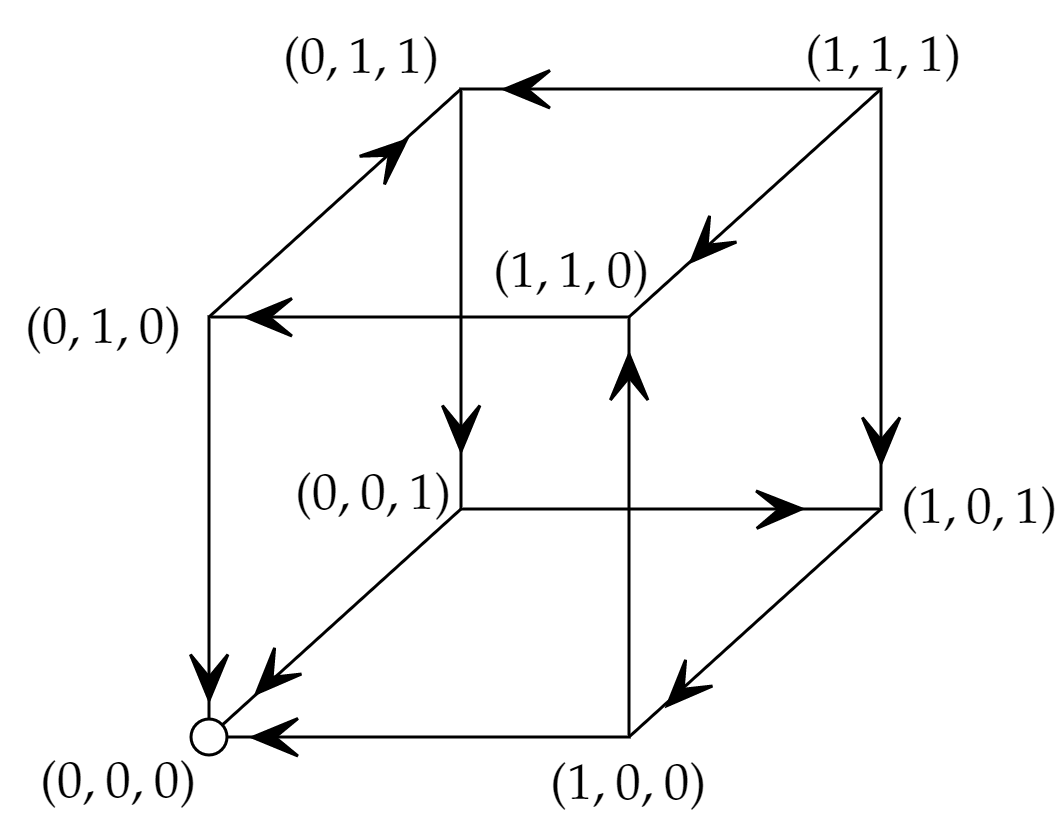
\includegraphics[width=0.45\linewidth]{USO.png}
        \caption{Одностоковая ориентация трехмерного булева куба $\BB_3$}
    \end{figure}
\end{frame}


\begin{frame}%{Граф семейства $\Gamma(F)$}
    Пусть $\ff$~--- семейство булевых функций.
    \begin{myexample}{Граф семейства $\Gamma_{\ff}$, \defn~47}
        \begin{coloritemize}
            \item Вершины: $V = \{ \alpha \in \EE_2^n \}$.
            \item Пусть $\alpha \ne \beta$, $\rho(\alpha, \beta) = 1$, $\alpha_i \ne \beta_i$, добавим ориентированное ребро $(\beta, \alpha) \in E$ тогда и только тогда, когда $f_i(\alpha) = \alpha_i$.
        \end{coloritemize}
    \end{myexample}
    \begin{figure}
        \centering
        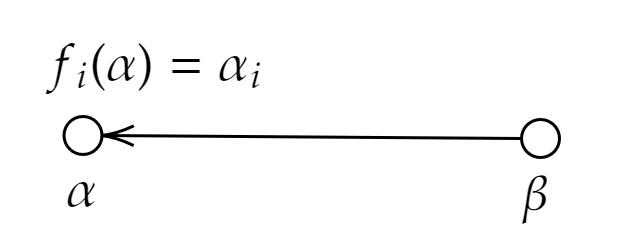
\includegraphics[width=0.45\linewidth]{edge.png}
    \end{figure}
\end{frame}


\begin{frame}{Стоки графа $\Gamma_{\ff}$}
    \begin{mytheorem}{Неподвижные точки булевых семейств, \lem~1}
        У правильного семейства булевых функций всегда существует единственная неподвижная точка.
    \end{mytheorem}
    \begin{coloritemize}
        \item  Неподвижная точка $\alpha$ отображения $x \to \ff(x)$ соответствует стоку в графе $\Gamma_{\ff}$ 
        \[
            f_i(\alpha) = \alpha_i, \quad 1 \le i \le n.
        \]
        \pause 
        \item Ориентации подкубов в $\Gamma_{\ff}$ задаются проекциями $\ff'$ семейства $\ff$.
    \end{coloritemize}
    \begin{mytheorem}{Взаимно-однозначное соответствие, \thm~9}
        Граф $\Gamma_{\ff}$ семейства булевых функций $\ff$ является одностоковой ориентацией ($\uso$) тогда и только тогда, когда $\ff$~--- правильное семейство.
    \end{mytheorem}
\end{frame}


\begin{frame}{$\uso$ и правильность: два описания одного объекта}  
    \begin{coloritemize}
        \item Существует взаимно-однозначное соответствие между \textquote{алгебраическим} (определение правильности) и \textquote{геометрическим} ($\uso$) описаниями.
        \item Это позволяет переводить результаты с одного \textquote{языка}на другой.
        \item Некоторые примеры переноса: вероятностный алгоритм порождения правильных семейств с помощью процедуры MCMC~\footcite{USOphd, galatenko21generation}, оценка на число булевых правильных семейств~\footcite{dm21}, новые классы правильных семейств.
    \end{coloritemize}    
\end{frame}


\begin{frame}
    Пусть $T(n)$ ($\Delta(n)$)~--- число \textbf{булевых} правильных (треугольных) семейств размера~$n$.
    \begin{mypropos}{Оценка на число булевых правильных семейств, \propos~23}
        \[
            n^{A \cdot 2^n} \le T(n) \le n^{B \cdot 2^n},
        \]
        где $A$, $B$~--- некоторые положительные константы.
        \footcitetext{numberUSO}
    \end{mypropos}
    \pause 
    \begin{mytheorem}{Булевых треугольных семейств экспоненциально мало, \thm~10}
        \[
            \frac{\Delta(n)}{T(n)} = o \Big(\frac{1}{n^{D \cdot 2^n}} \Big) \text{ при } n \to \infty,
        \]
        для некоторого $D > 0$.
        Почти все булевы правильные семейства не являются треугольными.
    \end{mytheorem}
\end{frame}


\begin{frame}{Рекурсивная треугольность}
    \begin{myexample}{Рекурсивно треугольное семейство, \defn~48}
        Семейство $\ff \colon \EE_k^n \to \EE_k^n$ со свойством: существует $i$, такое что $f_i \equiv const_i$, и $\proj_a^i(\ff)$ рекурсивно треугольны для всех $a \in \EE_k$.
    \end{myexample}
    Обобщение понятия рекурсивной ориентации булева куба~\footnote{\cite[A141770]{oeis}}.
    \pause
    Треугольные семейства являются рекурсивно треугольными.
    \pause
    \begin{mytheorem}{О правильности рекурсивно треугольных семейств, \lem~9}
        Рекурсивно треугольные семейства являются правильными.
    \end{mytheorem}
    \pause 
    Теорема доказывается через локально треугольные семейства, о них позднее.
\end{frame}


\begin{frame}{Рекуррентное соотношение}
    \begin{mytheorem}{Рекурсивно треугольных семейств мало, \lem~5, \thm~11}
        Пусть $\Delta^{\rec}_k(n)$~--- число рекурсивно треугольных семейств размера~$n$ над $k$-значной логикой.
        Тогда выполняется равенство:
        \[
            \Delta^{\rec}_k(n) = \sum_{j=1}^{n} (-1)^{j+1} \cdot k^j \cdot {n \choose j} \Delta^{\rec}_k(n-j)^{k^j}.
        \]

        Доля булевых рекурсивно треугольных семейств размера $n$ в классе всех булевых правильных семейств размера $n$ стремится к 0 при $n \to \infty$.
    \end{mytheorem}
    Обобщение результата для рекурсивной ориентации булева куба~\footnote{\cite[A141770]{oeis}}.
\end{frame}


\begin{frame}{Неподвижные точки правильного семейства}
    \begin{mytheorem}{\textbf{Следствие}~1}
        Булево семейство $\ff$ является правильным тогда и только тогда, когда семейство $\ff$ и каждая из его проекций имеет единственную неподвижную точку.
    \end{mytheorem}
    \pause 

    В общем случае: семейство $\ff \colon \EE_k^n \to \EE_k^n$ является правильным тогда и только тогда, когда для любой перекодировки $\ff$ все её проекции имеют единственную неподвижную точку~\footcite{galatenko21criterion}.

    \pause 
    В булевом случае свойство единственности неподвижной точки дает ещё одно характеристическое свойство правильных семейств, которое изучалось в контексте математической биологии (экспрессия генов~\footcite{thomas1991regulatory, richard2015fixed, ruet2015asynchronous, ruet2016local}).
\end{frame}


\begin{frame}%{$\hupf$-сети}
    \begin{myexample}{Булевы сети с наследственно единственной неподвижной точкой, \defn~}
        $\hupf$-сеть (сеть с наследственно единственной неподвижной точкой, hereditarily unique fixed point network)~--- булево семейство $\ff$ со следующим свойством: $\ff$ и все его проекции имеют единственную неподвижную точку (как отображения $\EE_2^n \to \EE_2^n$).
        \footcitetext{richard2015fixed}
    \end{myexample}
    \pause 
    \begin{mytheorem}{Правильные семейства $\leftrightarrow$ $\hupf$-сети, \thm~12}
        Булево семейство $\ff$ является правильным $\Leftrightarrow$ $\ff$ задает $\hupf$-сеть. 
    \end{mytheorem}
    Соответствие между булевыми правильными семействами и $\hupf$-сетями позволяет перенести (и обобщить) часть результатов, полученных в контексте изучения динамики таких сетей, на правильные семейства.
\end{frame}


\begin{frame}%{Локальный граф взаимодействий}
    Пусть $\ff$~--- семейство размера $n$.
    \begin{myexample}{{Локальный граф взаимодействий $G(\ff, \alpha)$}}
        \begin{coloritemize}
        \item Вершины: $V = \{1, \ldots, n\}$.
        \item Ребра: $i \to j$ тогда и только тогда, когда $f_j$ существенно зависит от $x_i$  \textquote{локально} в точке $a$:
        \[
            f_j(\alpha_1, \ldots, \alpha_i, \ldots, \alpha_n) \ne f_j(\alpha_1, \ldots, \alpha_i \oplus 1, \ldots, \alpha_n).
        \]
        \end{coloritemize}
    \end{myexample}
    \pause 
    \begin{mypropos}{Ациклические локальные графы}
        Пусть $G(\ff, \alpha)$~--- ациклический для каждой точки $\alpha \in \EE_2^n$, тогда $\ff$~--- $\hupf$-сеть.
        \footcitetext{shih2005combinatorial}
    \end{mypropos}
\end{frame}


\begin{frame}{Локальный граф взаимодействий-2}
    \begin{myexample}{Локально треугольные семейства, \defn~51}
        $\ff \colon \EE_k^n \to \EE_k^n $ локально треугольно, если $G(\ff, \alpha)$ ацикличен для каждой точки $\alpha \in \EE_k^n$, где локальная зависимость $f$ от $x_i$ в точке $\alpha$ определяется неравенством:
        \[
            \exists b \colon f(\alpha_1, \ldots, \alpha_i, \ldots, \alpha_n) \ne f(\alpha_1, \ldots, b, \ldots, \alpha_n).
        \]
    \end{myexample}
    \pause 
    \begin{mytheorem}{\thm~13}
        Локально треугольные семейства являются правильными.
    \end{mytheorem}
    Обобщение результата~\footcite{shih2005combinatorial} на $k$-значную логику.
    \pause 
    \begin{mytheorem}{\lem~9}
        Всякое рекурсивно треугольное семейство является локально треугольным.
    \end{mytheorem}
\end{frame}


\begin{frame}{Характеризация через несамодвойственные проекции}
    \begin{block}{Самодвойственное семейство}
        Отображение $\ff \colon \EE_2^n \to \EE_2^k$ самодвойственно, если для любого набора $x \in \EE_2^n$ выполняется свойство $\ff(\overline{x}) = \overline{\ff(x)}$.
    \end{block}
    \pause 
    \begin{mytheorem}{О несамодвойственности проекций, \thm~14} 
        Семейство $\ff$ булевых функций правильно тогда и только тогда, когда каждая из его проекций 
        \[
            \proj^{a_1, \ldots, a_k}_{i_1, \ldots, i_k}(\ff)
        \] 
        \textbf{не является} самодвойственным булевым отображением.
    \end{mytheorem}
    По сути~--- следствие результата из~\cite{richard2015fixed}.
\end{frame}


\begin{frame}{Кликовое представление правильных семейств}
    \begin{coloritemize}
        \item Правильные семейства находятся во взаимно-однозначном соответствии с кликами некоторым образом построенного графа (\textquote{обобщенный граф Келлера}).
        \pause
        \item Для $k=2$ перенос из теории $\mathsf{USO}$-ориентаций~\footcite{borzechowski2022universal}, для $k > 2$~--- авторское обобщение.
        \pause
        \item Обобщенный граф Келлера $G(k, n)$: $V = \EE_{k^2}^n$, 
        \[
            \{v, w\} \in E \leftrightarrow \exists i, \, 1 \le i \le n \colon v_i \equiv w_i \text{ mod } \; k, \; v_i \ne w_i.
        \]
        \pause
        \item Графы примечательны тем, что в случае $k = 2$ некоторым образом кодируют неэквивалентные замощения пространства гиперкубами~\footcite{sikiric2007cube, mathew2013enumerating}.
    \end{coloritemize}
    \pause
    \begin{mytheorem}{\thm~15}
        Каждой клике на $k^n$ вершинах в графе $G(k, n)$ можно поставить в биективное соответствие некоторое правильное семейство $\ff_n$ размера $n$ на $\EE_k^n$.
    \end{mytheorem}
\end{frame}


\section{Глава 3: свойства правильных семейств}

\begin{frame}{Общий вид биекций, сохраняющих правильность}
    Сдвиги, согласованные перенумерации, перекодировки~--- все эти преобразования:
    \begin{coloritemize}
        \item биективны,
        \pause 
        \item сохраняют правильность семейства,
        \pause 
        \item являются изометриями $\EE_k^n$ (в метрике Хэмминга).
    \end{coloritemize}

    \pause
    Общая постановка задачи: пусть $\Phi$, $\Psi$~--- биекции на $Q^n$: $\Phi, \Psi \in Perm(Q^n)$.
    Рассмотрим стабилизатор множества всех правильных семейств, заданных на $Q^n$:
    \[
        \{(\Phi, \Psi) \in Perm(Q^n) \mid \Phi(F(\Psi(x))) \text{ правильно для любого правильного } F \colon Q^n \to Q^n \}.  
    \]
        
    \pause
    Описать структуру этого множества.
\end{frame}


\begin{frame}{Общий вид биекций, сохраняющих правильность}
    \begin{mytheorem}{Стабилизатор правильных семейств, \thm~19}
        Пусть семейства $\gf(\xx)$ вида $\gf(\xx) = \Phi(\ff(\Psi(\xx)))$ являются правильным для всех правильных семейств $\ff$, заданных на $\EE_k^n$, $\Phi$ и $\Psi$~--- биекции множества $\EE_k^n$.
        Тогда $\Phi$ и $\Psi$ имеют вид 
        \[
            \Phi = \sigma \circ A, \Psi = \sigma \circ B, 
        \]
        где использованы следующие обозначения:
        \begin{description}
            \item[$\sigma \in \SSS_n$:] перенумерация координат вектора,
            \item[$A, B \in \left( \SSS_{\EE_k} \right)^n$:] перекодировки вектора. 
        \end{description}
    \end{mytheorem}
\end{frame}


\begin{frame}{Связь мощности образа и числа порождаемых квазигрупп}
    Пусть $\ff = (f_1, \ldots, f_n)$~--- правильное, тогда отображение вида 
    \[
        (x, y) \to z = x \oplus y \oplus f(\pi_1(x_1, y_1), \ldots, \pi_n(x_n, y_n))
    \]
    задает квазигрупповую операцию \textbf{при любом выборе} $\pi_1, \ldots, \pi_n$.
    \pause 
    \begin{coloritemize}
        \item Сколько может получиться \textbf{различных} квазигрупп при разных $\pi_1, \ldots, \pi_n$?
        \pause 
        \item Плохой пример: если все $f_i \equiv const_i$, то смена $\pi_i$ ничего не даст.
    \end{coloritemize}
    \begin{mypropos}{\propos~2}
        Пусть $\ff \colon \EE_k^n \to \EE_k^n$~--- правильное семейство, $M$~--- мощность образа отображения $x \to \ff(x)$.
        Тогда число различных квазигрупп, порождаемых указанной конструкцией, не менее чем $M^{k^2}$.
        \footcitetext{galatenko23}
    \end{mypropos}
\end{frame}


\begin{frame}
    \begin{mypropos}{Ограниченность мощности образа, \propos~29}
        Число значений, принимаемых правильным семейством порядка~$n$ в $k$-значной логике, не превосходит~$k^{n-1}$.
        \footcitetext{galatenko23}
    \end{mypropos}
    \pause 
    \begin{mytheorem}{Мощность образа квадратичного семейства, \thm~21}
        Семейство 
        \[
            \begin{bmatrix}
            0 \\
            x_1 \\
            \vdots \\
            x_1 \oplus x_2 \oplus \ldots \oplus x_{n-1}
            \end{bmatrix}
            \bigoplus
            \begin{bmatrix}
            \bigoplus_{i < j, \; i, j \ne 1}^n \; x_i x_j \\
            \bigoplus_{i < j, \; i, j \ne 2}^n \; x_i x_j \\
            \vdots \\
            \bigoplus_{i < j, \; i, j \ne n}^n \; x_i x_j \\
            \end{bmatrix}
        \]
        имеет максимальную мощность образа~$2^{n-1}$.
    \end{mytheorem}
\end{frame}


\begin{frame}%{Мощности образов некоторых конкретных правильных семейств-2}
    \[
        \ff_n(x) = 
        \begin{bmatrix}
            f_1(x_1, \ldots, x_n) \\
            f_2(x_1, \ldots, x_n) \\
            \vdots \\
            f_n(x_1, \ldots, x_n) \\
        \end{bmatrix}
        =
        \begin{bmatrix}
            \overline{x}_2 \cdot x_3 \\
            \overline{x}_3 \cdot x_4 \\
            \vdots \\
            \overline{x}_1 \cdot x_2 \\
        \end{bmatrix}.
    \]
    \begin{mypropos}{Правильность семейства, \rema~17}
        Семейство $\ff_n$ является правильным при нечетных $n$.
        \footcitetext{galatenko20quad}
    \end{mypropos}
    \pause
    \begin{mytheorem}{Мощность образа семейства, \thm~22}
        Мощность образа семейства $\ff_n$ равна $\lucas_n$ ($n$-е число Люка):
        \[
            \lucas_n = \lucas_{n-1} + \lucas_{n-2}, \quad \lucas_0 = 2, \quad \lucas_1 = 1.
        \]
    \end{mytheorem}
\end{frame}


\begin{frame}{Подстановки, порождаемые правильными семействами}
    Пусть $\ff \colon Q^n \to Q^n$~--- правильное, $(Q, \circ)$~--- квазигруппа.
    Тогда отображение
    \[ 
        \sigma_\ff(x) \colon x \to x \circ \ff(x),
        \quad
        \begin{bmatrix}
            x_1 \\
            \vdots \\
            x_n
        \end{bmatrix} 
        \to 
        \begin{bmatrix}
            x_1 \circ f_1(x_1, \ldots, x_n) \\
            \vdots \\
            x_n \circ f_n(x_1, \ldots, x_n)
        \end{bmatrix}
    \]
    является подстановкой: $\sigma_{\ff} \in Perm(Q^n)$.
\end{frame}


\begin{frame}
    Пусть $\ff \colon Q^n \to Q^n$~--- правильное.
    Рассмотрим $\sigma^{-1}_{\ff} \in Perm(Q^n)$.
    \begin{mytheorem}{Обратимость \textquote{правильных подстановок}, \thm~23}
        Если $(Q, +)$~--- группа (т.е., операция $+$ ассоциативна), то семейство $\gf \colon Q^n \to Q^n$, определенное равенством
        \[
            \gf(x) = (-x) + \sigma_{\ff}^{-1}(x)
        \]
        также является правильным.
    \end{mytheorem}
    \pause
    Т.е., если $\ff$~--- правильное, то существует правильное семейство $\gf$ со свойством
    \[
        \sigma^{-1}_{\ff}(x) = \sigma_{\gf}(x).
    \]
    \pause
    Таким образом, множество \textquote{правильных подстановок} замкнуто относительно взятия обратного элемента (в случае, когда $Q$~--- группа).
\end{frame}


\begin{frame}{О подстановках, порождаемых правильными семействами-2}
    Множество \textquote{правильных подстановок}$\sprop$ \textbf{не является} подгруппой $Perm(Q^n)$.
    
    \pause 
    \begin{mytheorem}{Транзитивность действия, \thm~25}
        Замыкание $\sprop$ действует транзитивно на $Q^n$ (любой элемент из $Q^n$ можно перевести в любой другой с помощью композиции некоторого количества $\sigma_{F}$).
    \end{mytheorem}
    \pause 
    \begin{mypropos}{Булев случай}
        При $Q = \EE_2$ замыкание $\sigma_{\ff}$ порождает все множество подстановок $Perm(\EE_2^n)$.
        \footcitetext{USOphd}
    \end{mypropos}
\end{frame}


\begin{frame}{О подстановках, порождаемых правильными семействами-3}
    Пусть $\ff$~--- правильное семейство булевых функций.
    \begin{mytheorem}{Четность числа элементов в прообразе, \thm~20}
    \label{thm:preimage}
        Для любого $\alpha \in \{0, 1\}^n$ число решений уравнения $\ff(x) = \alpha$ всегда четно.
    \end{mytheorem}
    \pause
    \begin{mytheorem}{Количество неподвижных точек $\sigma_{\ff}$, \thm~24}
        У подстановки $\sigma_{\ff}(x) = x \oplus {\ff}(x)$ чётное число неподвижных точек.
    \end{mytheorem}
\end{frame}


\section{Глава 4: алгоритмические и вычислительные аспекты}


\begin{frame}{Алгоритм шифрования, сохраняющего формат ($\fpe$-схема)}
    \begin{coloritemize}
        \item $\fpe$-схема~\footcite{bellare2009format}: алгоритм, позволяющий зашифровывать сообщения из произвольного конечного множества $M$ таким образом, что результат зашифрования также лежит в множестве $M$.
        \pause 
        \item Преобразуем $m \in M$, где $(M, \circ)$~--- квазигруппа, в $c \in M$ по правилу:
        \[
            m \to c = L_{k_1, \ldots, k_{\ell}}(m) = k_1 \circ \left( k_2 \circ ( \ldots ( k_{\ell} \circ m) \ldots ) \right).
        \]
        \pause 
        \item Элементы $k_i$ и последовательность сдвигов выбирается на основе мастер-ключа и настройки (tweak) псевдослучайным образом.
        \pause 
        \item Необходимо специфицировать конкретную квазигруппу.
    \end{coloritemize}
\end{frame}


\begin{frame}
    \begin{coloritemize}
        \item Пусть $\ff$, $\gf$~--- правильные семейства на $(H^n, +)$.
        \pause 
        \item Рассмотрим квазигруппу 
        \[
            (x, y) \to x \circ y = x + \ff(x) + y + \gf(y),
        \]
        \pause
        \item Если $\ff$~--- правильное семейство на группе $H^n$, то семейство $\widetilde{\ff}$
        \[
            \widetilde{\ff}(x) = (-x) + \pi^{-1}_{\ff}(x), \quad \pi_{\ff}(x) = x + \ff(x), \quad x \in H^n,
        \]
        также является правильным на $H^n$.
        \pause
        \item Таким образом, операция $x \circ y$ \textbf{обращается справа} следующим образом:
        \[
            x = \pi_{\widetilde{F}} \left( (x \circ y) - \pi_G(y) \right).
        \]
        \pause 
        \item Обращение слева также возможно.
        \pause 
        Обращение $\Leftrightarrow$ алгоритм расшифрования $\Leftrightarrow$ $\fpe$-схема.
    \end{coloritemize}
\end{frame}


\begin{frame}{Сложность распознавания правильности}
    \begin{coloritemize}
        \item В общем случае проверка правильности является сложной задачей: если семейство задано в форме КНФ, то задача проверки правильности coNP-полна~\footcite{nosov98}.
        \pause 
        \item В определенных случаях задача проверки правильности может быть упрощена, в частности, за счет вида графа существенной зависимости~\footcite{rykov14}.
        \pause 
        \item Алгоритм проверки правильности булева семейства требует порядка $\Theta(4^n)$ операций вычисления правильного семейства на двоичном наборе $x$ (проверка по определению правильности).
        \pause 
        \item Предложена адаптация алгоритма~\footcite{bosshard2017pseudo} со сложностью $\Theta(3^n)$, проверяющего, что ориентация $\Gamma_{\ff}$, задаваемая семейством $\ff$, является одностоковой.
        \pause 
        \item Алгоритм опирается на характеристическое свойство правильных семейств: булево семейство правильно тогда и только тогда, когда каждая его проекция не является самодвойственным отображением.
    \end{coloritemize}
\end{frame}


\begin{frame}{Численные эксперименты}
    \begin{center}
        \begin{tabular}{|c|c|c|c|c|}
            \hline
            Размер $n$  & $\Delta(n)$ & $\Delta^{\rec}(n)$ & $\Delta^{\loc}(n)$ & $T(n)$ \\
            \hline
            $n = 1$ & 2 & 2 & 2 & 2 \\
            \hline
            $n = 2$ & 12 & 12 & 12 & 12 \\
            \hline
            $n = 3$ & 488 & 680 & 680 & 744\\
            \hline
            $n = 4$ & 481776 & 3209712 & 3349488 & 5541744 \\
            \hline
            $n = 5$ & 157549032992 & 94504354122272 & --- & 638560878292512 \\
            \hline
        \end{tabular}


        $\Delta(n)$: число булевых треугольных семейств размера $n$;
        $\Delta^{\loc}(n)$: число булевых локально-треугольных семейств размера $n$;
        $\Delta^{\rec}(n)$: число булевых рекурсивно-треугольных семейств размера $n$;
        $T(n)$: число булевых правильных семейств размера $n$.
    \end{center}
\end{frame}


\begin{frame}{Число классов эквивалентности}
    \begin{center}
        \begin{tabular}{|c|c|c|}
            \hline
            Размер $n$ & Число классов 1 & Число классов 2 \\
            \hline
            $n = 1$ & 1 & 1 \\
            \hline
            $n = 2$ & 2 & 2 \\
            \hline
            $n = 3$ & 19 & 10 \\
            \hline
            $n = 4$ & 14614 & 1291 \\
            \hline
        \end{tabular}

        Классы 1 (2): классы отношения эквивалентности, заданного согласованными подстановками совместно с (внутренними и) внешними сдвигами.
    \end{center}
\end{frame}


\begin{frame}{Индексы ассоциативности, $n=2$}
    \begin{center}
        \begin{tabular}{|c|c|}
            \hline
            $a(Q)$ & Кол-во $Q$ \\
            \hline
            16 & 32 \\
            \hline
            32 & 96 \\
            \hline
            64 & 16 \\
            \hline
        \end{tabular}
        \; \par 
        \; \par
        Квазигруппа $Q = (\EE_2^n, \circ)$ задается по паре правильных булевых семейств $\ff$, $\gf$ с помощью операции
        \[
            (x, y) \to x \circ y = x + \ff(x) + y + \gf(y).
        \]
    \end{center}
\end{frame}


\begin{frame}{Индексы ассоциативности, $n=3$}
    \begin{center}
        \begin{tabular}{|c|c|c|c|}
            \hline
            $a(Q)$ & Кол-во $Q$ & $a(Q)$ & Кол-во $Q$ \\
            \hline
            64 & 27648 & 144 & 3072\\
            80 & 103424 & 160 & 84480 \\
            88 & 18432 & 176 & 6144\\
            96 & 82944 & 192 & 18432\\
            104 & 33792 & 208 & 3072\\
            112 & 21504 & 256 & 10368\\
            120 & 21504 & 320 & 2304\\
            128 & 116352 & 512 & 64\\
            \hline
        \end{tabular}
    \end{center}
\end{frame}


\begin{frame}{Индексы ассоциативности, $n=4$}
    \begin{columns}[T] % gather columns
        \begin{column}{.49\textwidth}
            \begin{figure}[h]
                \centering 
                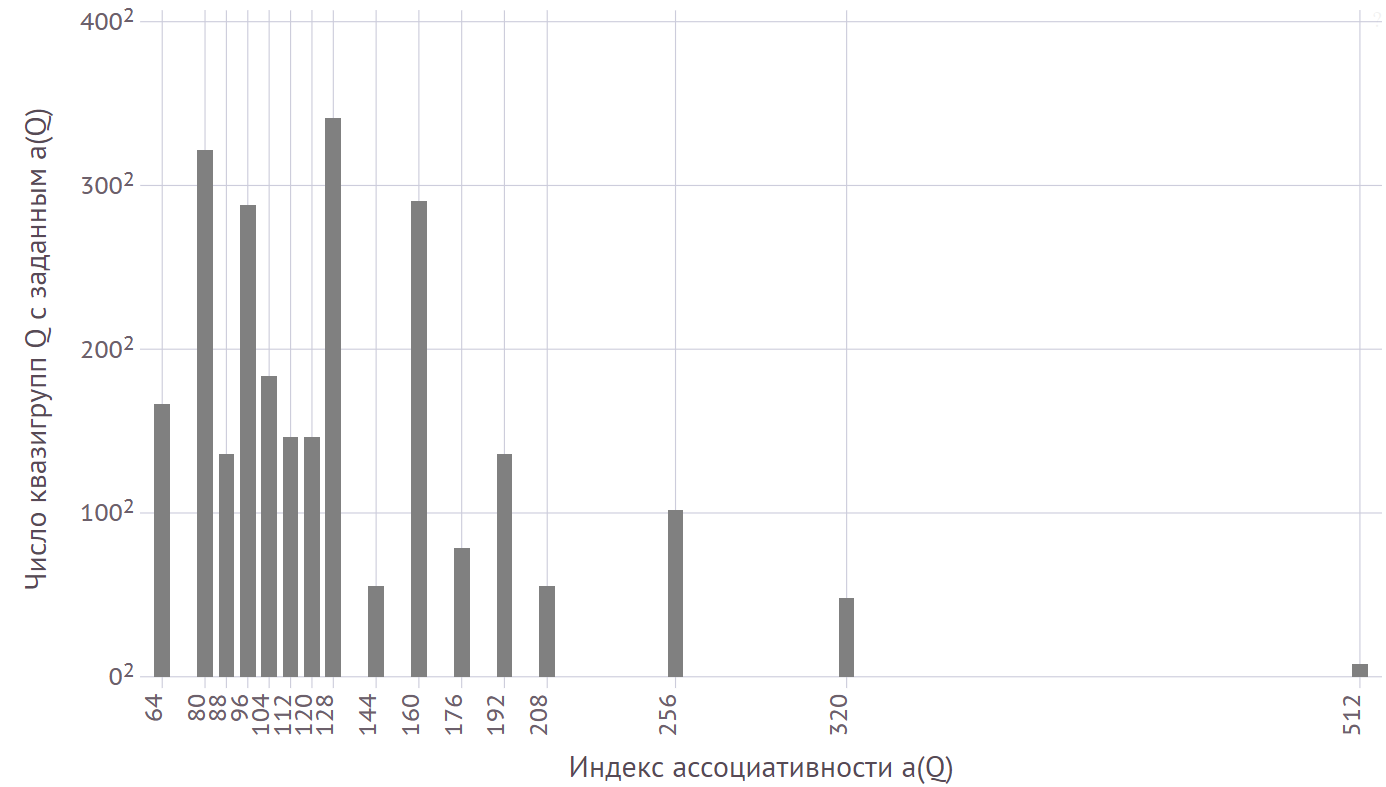
\includegraphics[scale = 0.4]{histogram.png}
            \end{figure}
        \end{column}%
        \hfill%
        \begin{column}{.49\textwidth}
            \begin{figure}[h]
                \centering 
                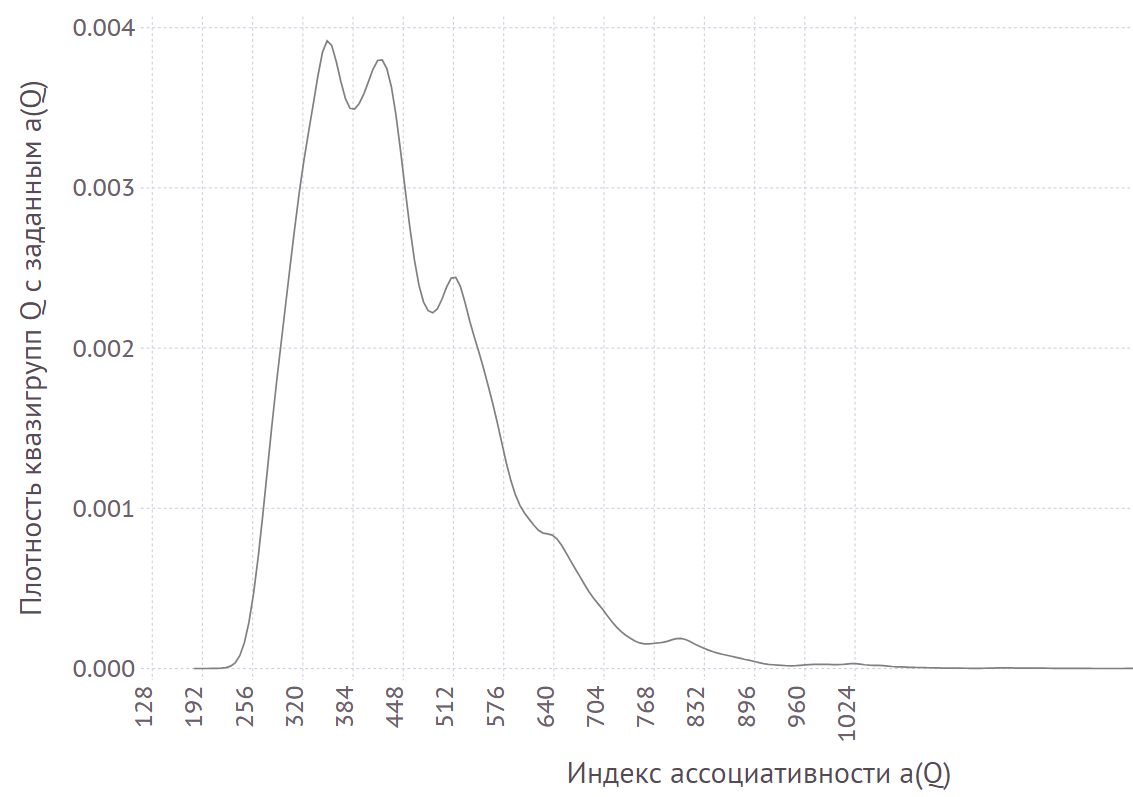
\includegraphics[scale = 0.4]{density.png}
            \end{figure}
        \end{column}%
    \end{columns}  
\end{frame}


\begin{frame}{Основные результаты диссертации}
    \begin{coloritemize}
        \item Установлено естественное соответствие между булевыми правильными семействами и одностоковыми ориентациями графов булевых кубов ($\uso$-ориентации), а также между булевыми правильными семействами и булевыми сетями с наследственно единственной неподвижной точкой ($\hupf$-сети); установлено естественное соответствие между правильными семействами в логике произвольной значности и кликами в обобщенных графах Келлера.
        \pause 
        \item Доказано, что стабилизатором множества правильных семейств функций являются изометрии пространства Хэмминга (согласованные перенумерации и перекодировки); показано, что отображения, задаваемые с помощью правильных семейств булевых функций, всегда имеют четное число неподвижных точек; 
        получена оценка на число правильных семейств булевых функций, предложены оценки доли треугольных семейств среди всех правильных семейств булевых функций.
        \end{coloritemize}
\end{frame}


\begin{frame}{Основные результаты диссертации-2}
    \begin{coloritemize}
        \item Построены новые классы правильных семейств функций (рекурсивно треугольные, локально треугольные, сильно квадратичное семейство); получены оценки на число рекурсивно треугольных семейств; для некоторых правильных семейств булевых функций получены точные значения мощности образа отображений, задаваемых этими правильными семействами.
        \pause
        \item Предложен новый способ порождения квазигрупп на основе правильных семейств функций; доказан ряд утверждений о числе ассоциативных троек в порождаемых квазигруппах; предложен новый алгоритм шифрования, сохраняющего формат ($\fpe$-схема), основанный на квазигрупповых операциях.
    \end{coloritemize}
\end{frame}


\begin{frame}{Публикации автора (личные)}
    \begin{coloritemize}
        \item \textquote{О соответствии между правильными семействами и реберными ориентациями булевых кубов}, Интеллектуальные системы. Теория и приложения, 24:1 (2020), 97--100.
        \item \textquote{О взаимно однозначном соответствии между правильными семействами булевых функций и рёберными ориентациями булевых кубов}, ПДМ, 2020, 48,  16--21 (2020).
        \item \textquote{О свойствах правильных семейств булевых функций}, Дискрет. матем., 33:1 (2021), 91--102.
        \item ``Format-preserving encryption: a survey'', Матем. вопр. криптогр., 13:2 (2022),  133--153.
        \item \textquote{Об одном квазигрупповом алгоритме шифрования, сохраняющего формат}, ПДМ. Приложение, 2023, 16,  102--104.
        \item \textquote{Об индексе ассоциативности конечных квазигрупп}, Интеллектуальные системы. Теория и приложения, 28:3 (2024), 80--101. 
    \end{coloritemize}
\end{frame}


\begin{frame}{Публикации автора (в соавторстве)}
    \begin{coloritemize}
        \item A. V. Galatenko, V. A. Nosov, A. E. Pankratiev, K. D. Tsaregorodtsev, ``Proper families of functions and their applications'', Матем. вопр. криптогр., 14:2 (2023),  43--58.
        \item А. В. Галатенко, В. А. Носов, А. Е. Панкратьев, К. Д. Царегородцев, \textquote{О порождении n-квазигрупп с помощью правильных семейств функций}, Дискрет. матем., 35:1 (2023),  35--53.
        \item A. V. Galatenko, A. E. Pankratiev, K. D. Tsaregorodtsev,``A Criterion of Properness for a Family of Functions'', Journal of Mathematical Sciences, 284:4 (2024), 451--459.
    \end{coloritemize}
\end{frame}